\subsubsection{UC2 - Errore per fallita autenticazione}\label{UC2}

\begin{figure}[H]
  \centering
  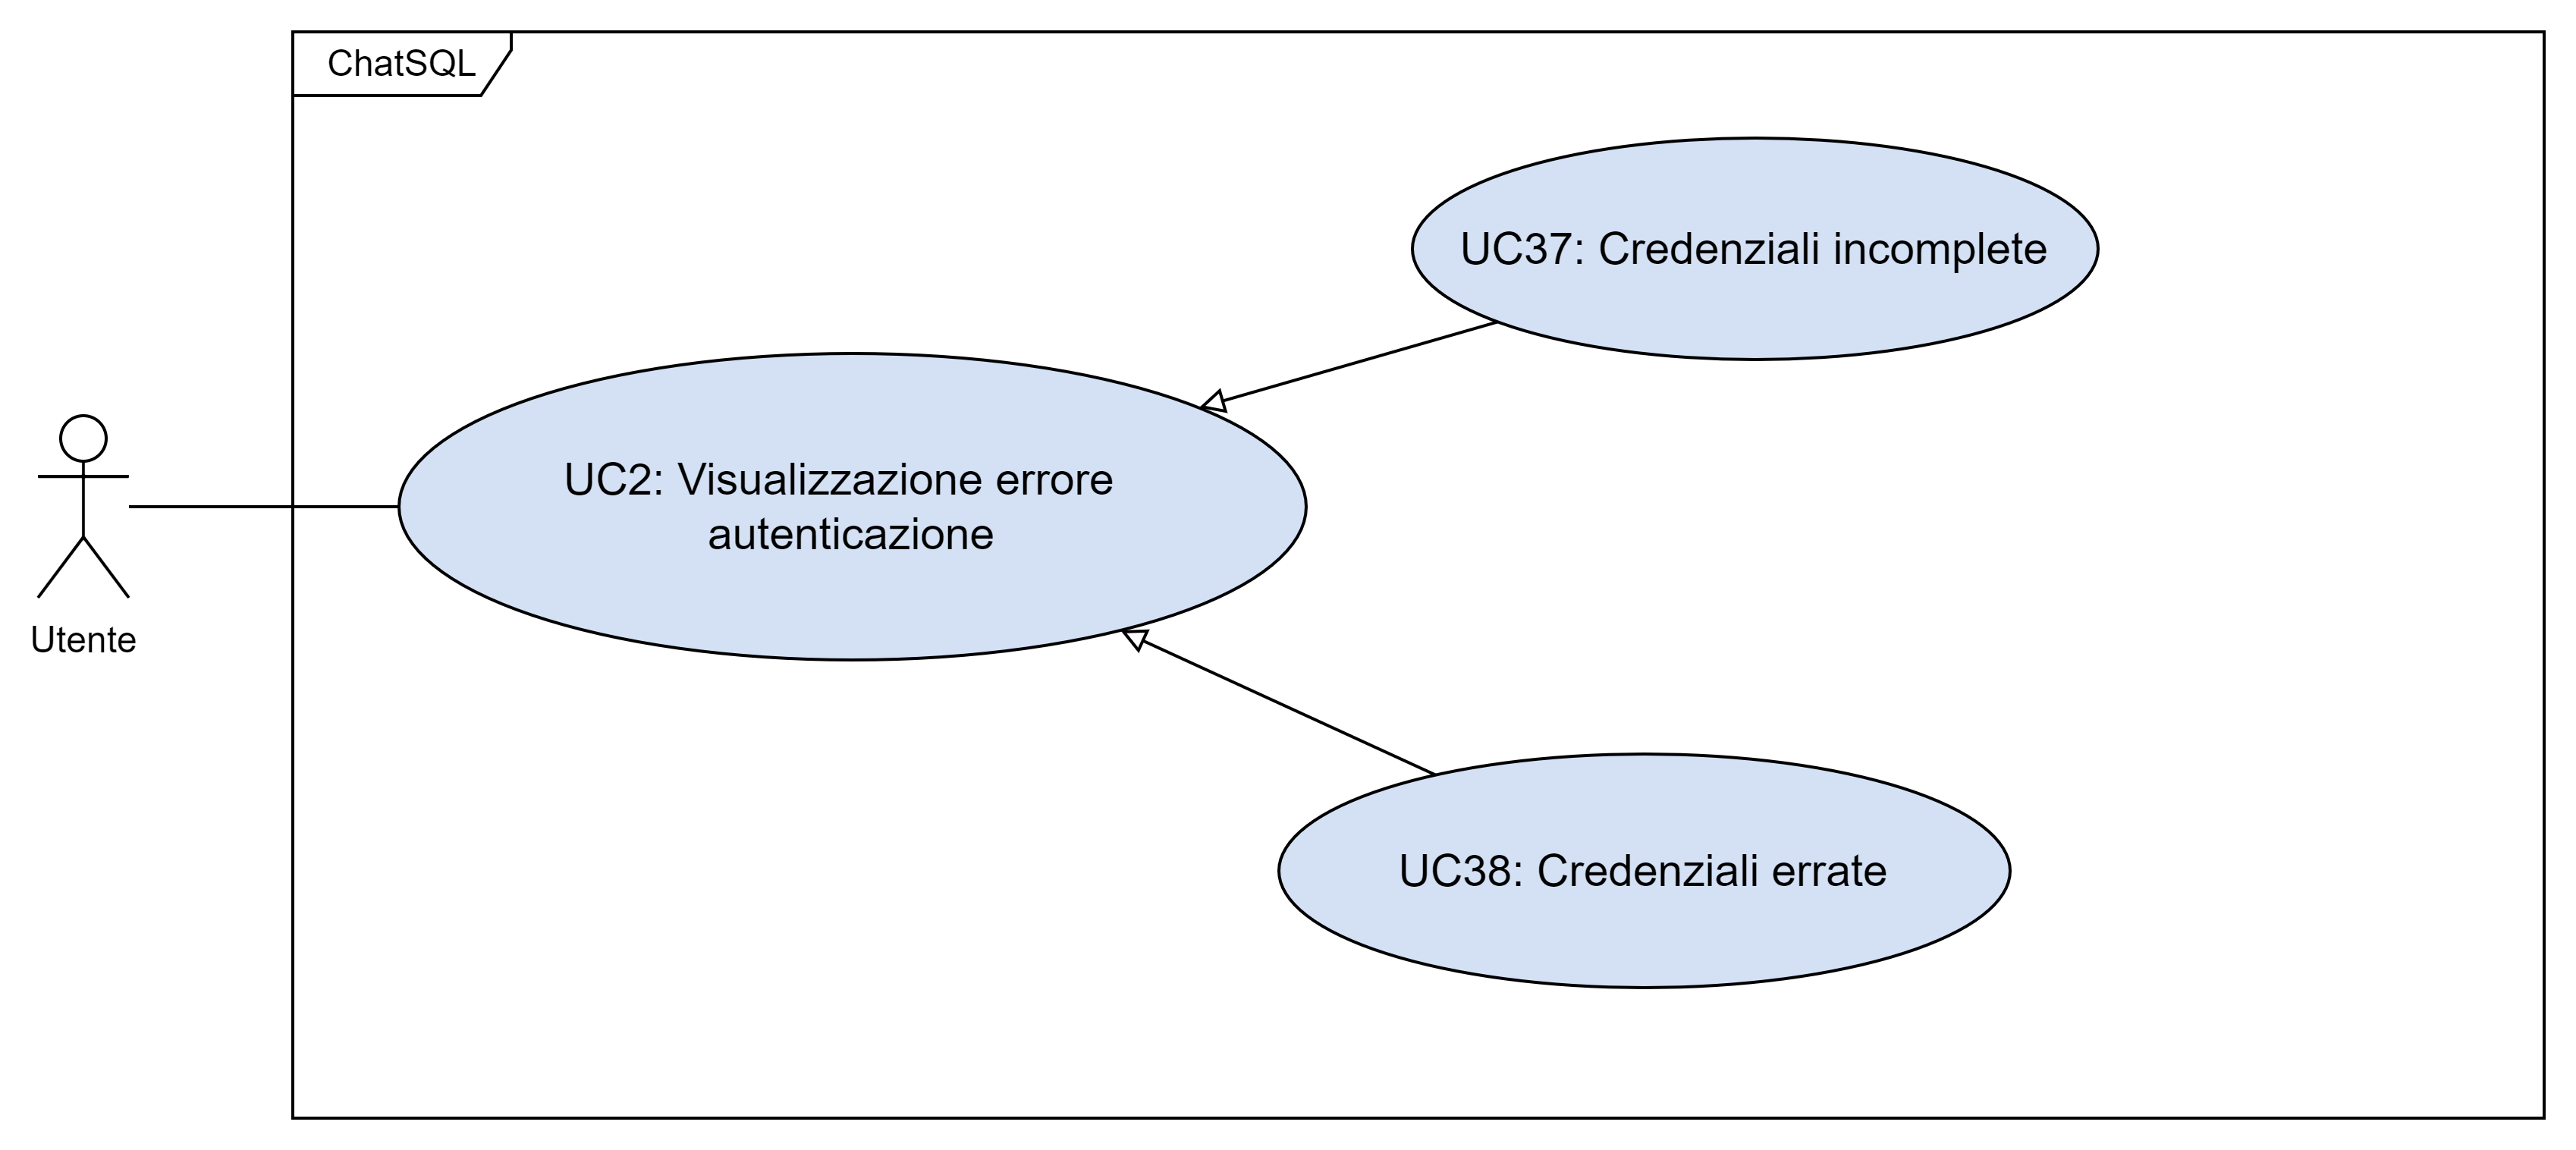
\includegraphics[width=0.90\textwidth]{assets/uc2.png}
  \caption{UC2}
\end{figure}

\paragraph*{Descrizione}
Nel caso in cui il sistema riveli delle irregolarità durante la validazione delle credenziali utilizzate per il login, l'Utente viene informato della natura del problema tramite appositi messaggi di errore.

\paragraph*{Attori principali}
Utente

\paragraph*{Precondizioni}
\begin{itemize}
  \item Il sistema è attivo e funzionante;
  \item L'Utente ha inserito le proprie credenziali nell'area di login (\hyperref[UC1]{UC1});
  \item Il sistema ha riscontrato un problema nel processo di autenticazione.  
\end{itemize}

\paragraph*{Postcondizioni}
\begin{itemize}
  \item Il sistema notifica l'utente della mancata autenticazione mediante un messaggio di errore e lo invita a riprovare.
\end{itemize}

\paragraph*{Scenario principale}
\begin{enumerate}
  \item L'Utente tenta di autenticarsi inserendo le proprie credenziali nell'area di login;
  \item Il sistema riscontra un problema nella validazione delle credenziali di accesso;
  \item Viene restituito all'Utente un messaggio di errore relativo alla problematica riscontrata;
  \item Il sistema invita l'Utente a riprovare l'autenticazione.
\end{enumerate}

\paragraph*{Generalizzazioni}
\begin{itemize}
  \item Errore credenziali incomplete (\hyperref[UC2point1]{UC2.1});
  \item Errore credenziali errate (\hyperref[UC2point2]{UC2.2});
\end{itemize}

%%%%%%%%%%%%%%%%%%%%%%%%%%%%%%%%%%%%%%%%%%%%%%%%%%%%%%%%%%%%%%%%%%%%%%%%%%%%%%

\subsubsection{UC2.1 - Errore credenziali incomplete}\label{UC2point1}
\paragraph*{Descrizione}
Il sistema restituisce un apposito messaggio di errore nel caso in cui l'Utente provi a inserire delle credenziali incomplete in fase di autenticazione.

\paragraph*{Attori principali}
Utente

\paragraph*{Precondizioni}
\begin{itemize}
  \item L'Utente ha tentato di autenticarsi inserendo credenziali incomplete.  
\end{itemize}

\paragraph*{Postcondizioni}
\begin{itemize}
  \item Viene restituito correttamente un messaggio di errore per notificare l'Utente dell'inserimento incompleto dei dati nell'area di login.
\end{itemize}

\paragraph*{Scenario principale}
\begin{enumerate}
  \item L'Utente richiede l'autenticazione inserendo delle credenziali incomplete;
  \item L'Utente visualizza il messaggio di errore relativo al mancato inserimento dei dati di accesso.   
\end{enumerate}

%%%%%%%%%%%%%%%%%%%%%%%%%%%%%%%%%%%%%%%%%%%%%%%%%%%%%%%%%%%%%%%%%%%%%%%%%%%%%%

\subsubsection{UC2.2 - Errore credenziali errate}\label{UC2point2}
\paragraph*{Descrizione}
Il sistema restituisce un apposito messaggio di errore nel caso in cui l'Utente provi a inserire delle credenziali errate in fase di autenticazione.

\paragraph*{Attori principali}
Utente

\paragraph*{Precondizioni}
\begin{itemize}
  \item L'Utente ha tentato di autenticarsi inserendo credenziali errate.  
\end{itemize}

\paragraph*{Postcondizioni}
\begin{itemize}
  \item Viene restituito correttamente un messaggio di errore per notificare l'Utente che le credenziali inserite non sono corrette.
\end{itemize}

\paragraph*{Scenario principale}
\begin{enumerate}
  \item L'Utente richiede l'autenticazione inserendo delle credenziali errate;   
  \item L'Utente visualizza il messaggio di errore relativo all'errato inserimento dei dati di accesso.   
\end{enumerate}
